
\subsection{A Case-study on Llama-1}

\label{sec:llama_case_study}

We now consider evaluating if the LRs used by Llama-1 \cite{llama1} are "correct" according to our scaling laws. To do this we adopt the LLama-1 architecture (RMSnorm, Rope embeddings, and so on) and run small-scale experiments with token horizons 25B, 50B, and 100B and different LRs. Based upon these experiments, we find that values for \Cref{eq:powerlaw} are $B=\e{8.29}{-4}$ and $\beta=0.3$ (see \Cref{fig:7b} in \Cref{appendix:experimental_data}). We then extrapolate to find the optimal LR at 1T tokens, which comes out as \scinot{1.15}{-4}. LLama-1 used \scinot{3}{-4}, an LR which is too large by a factor of $>2.5$ according to our results. This methodology is visualized in \Cref{fig:llama_wrong}. The numerical values used for our predictions are also tabulated in \Cref{table:7b_fit} in \Cref{appendix:experimental_data}, where we also compare to predicting the optimal LR for LLama-1 using our scaling law from Eq. \Cref{eq:scaling_law}. If Llama used the wrong LR, what were the actual effects of this? We provide an estimate on the \textit{upper bound} for the validation loss penalty between the optimal and used learning rate in Llama-1 using the parabola fit at $D=100B$. $\Delta L=L(D=100B,LR=\optlr)-L(D=100B,LR=2.6\optlr)=0.027$. Note, this is an upper bound since the parabolas flatten with longer token horizons











\begin{figure}[]
\begin{center}
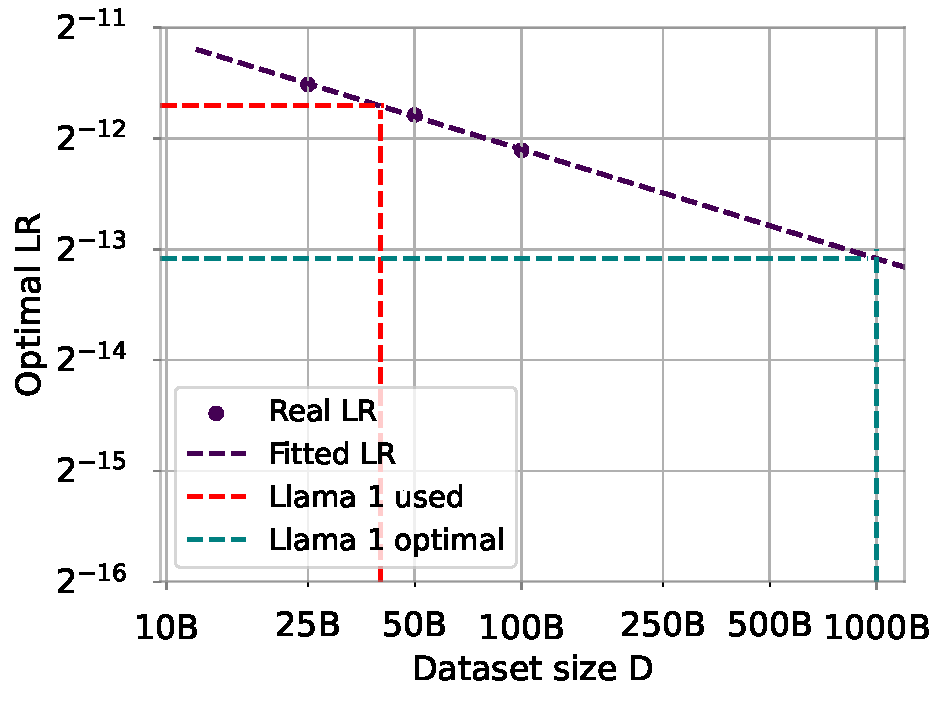
\includegraphics[width=0.6\textwidth]{images/llama_wrong.pdf}
\vspace{-0.3cm}
\caption{The optimal LR of the LLama-1 7B model as a function of token horizon $D$. We find that \scinot{1.15}{-4} is optimal for 1T tokens whereas the Llama-1 paper used \scinot{3}{-4}. \johan{minor/major ticks inconsistent pad. Make base-10?2}}
\vspace{-0.3cm}
\label{fig:llama_wrong}
\centering
\end{center}
\end{figure}



